El detector de marcadores de referencia se emplea en tres contextos operativos distintos dentro del sistema, demostrando la versatilidad y robustez del algoritmo desarrollado.\\

Aplicación 1: Corrección de posición horizontal\\
\noindent
En el contexto de corrección horizontal, el robot se posiciona frente a una cinta vertical y captura una imagen. El detector identifica la cinta y calcula la desviación horizontal del centroide respecto al centro de la imagen. Esta desviación, convertida a milímetros mediante calibración, se emplea para generar comandos de movimiento correctivo en el eje X que alinean el brazo precisamente con la cinta.

Este procedimiento se ejecuta posterior a que el robot haya detectado si la hay una planta lista para ser cosechada.\\

Aplicación 2: Corrección de posición vertical\\
\noindent
En el contexto de corrección vertical, el robot se posiciona sobre una cinta vertical y captura una imagen. El detector identifica la cinta y calcula la desviación vertical de la arista base de la cinta respecto al centro de la imagen. Esta desviación se emplea para generar comandos de movimiento correctivo en el eje Y que alinean verticalmente el brazo con la cinta.

Este procedimiento se ejecuta posterior a la corrección de posición horizontal par dejar alineado en ambos sentidos el robot previo a la cosecha.

\begin{figure}[H]
\centering
\begin{subfigure}[b]{0.48\textwidth}
    \centering
    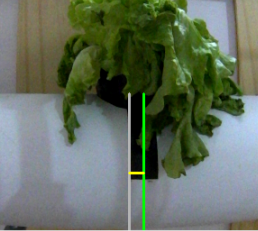
\includegraphics[width=\textwidth]{imagenes/detector_marcadores_5_lineas_verticales.png}
    \caption{Detección de cinta vertical para corrección horizontal}
\end{subfigure}
\hfill
\begin{subfigure}[b]{0.48\textwidth}
    \centering
    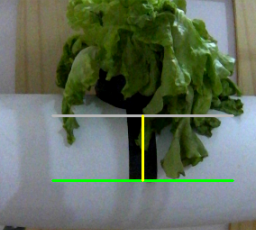
\includegraphics[width=\textwidth]{imagenes/detector_marcadores_5_lineas_horizontales.png}
    \caption{Detección de cinta horizontal para corrección vertical}
\end{subfigure}
\caption{\textit{Aplicaciones del detector de marcadores en ambos ejes de corrección}}
\label{fig:aplicaciones_marcadores}
\end{figure}

Aplicación 3: Escaneo horizontal para mapeo\\
\noindent
Durante la fase de mapeo autónomo del entorno, el robot recorre horizontalmente el espacio de trabajo detectando cintas verticales que marcan las posiciones de las estaciones de cultivo. El sistema opera en modo continuo mientras el robot se desplaza a velocidad reducida.

El procedimiento funciona mediante la adquisición de imágenes a 6 fotogramas por segundo durante el movimiento horizontal. Para cada frame capturado se ejecuta el algoritmo de detección de cintas. El sistema mantiene un seguimiento del estado de detección mediante flags:

Cuando el detector identifica una cinta en múltiples frames consecutivos (típicamente 5 frames para confirmar la detección), se envía un flag de inicio al nivel regulatorio que registra la coordenada X actual. Mientras el robot continúa avanzando y la cinta permanece visible, el sistema mantiene el estado de detección activo.

Cuando la cinta deja de detectarse durante varios frames consecutivos (típicamente 5 frames para confirmar la ausencia), se envía un flag de fin al nivel regulatorio que registra la nueva coordenada X. La posición de la cinta se calcula posteriormente como el promedio entre las coordenadas de inicio y fin registradas por ambos flags.

Este mecanismo con confirmación por frames consecutivos proporciona robustez ante falsos positivos ocasionales y permite mapear automáticamente todas las posiciones de cultivo sin conocimiento a priori de la geometría del sistema.